\documentclass{article}
\usepackage{amsmath}
\usepackage{pgfplots}
\pgfplotsset{compat=1.16}

\begin{document}

\begin{figure}[h]
    \centering
    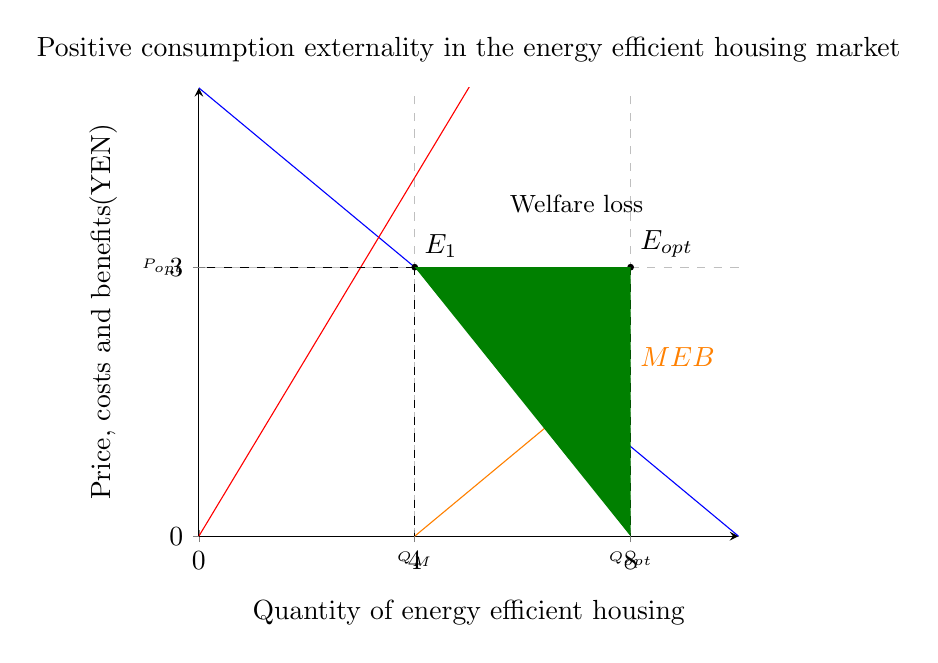
\begin{tikzpicture}
        \begin{axis}[
            axis lines = left,
            xlabel = {Quantity of energy efficient housing},
            ylabel = {Price, costs and benefits(YEN)},
            xmin=0, xmax=10,
            ymin=0, ymax=5,
            xtick={0,4,8},
            ytick={0,3},
            extra x ticks={4,8},
            extra x tick labels={$Q_M$, $Q_{opt}$},
            extra y ticks={3},
            extra y tick labels={$P_{opt}$},
            extra tick style={
                grid=major,
                ticklabel style={font=\tiny},
                grid style={dashed}
            },
            legend pos=north east,
            ymajorgrids=true,
            grid style=dashed,
            title={Positive consumption externality in the energy efficient housing market},
            title style={align=center},
            ]
            
            % Demand curve (MPB)
            \addplot[blue, domain=0:10, samples=100] {5 - 0.5*x} node[right] {$MSB$};
            
            % Supply curve (MPC = MSC)
            \addplot[red, domain=0:10, samples=100] {x} node[right] {$S = MPC = MSC$};
            
            % Marginal External Benefit (MEB)
            \addplot[orange, domain=4:8, samples=100] {0.5*(x-4)} node[right] {$MEB$};
            
            % Optimal Quantity (Q_opt) and Price (P_opt)
            \filldraw[black] (axis cs:8,3) circle (1pt) node[anchor=south west] {$E_{opt}$};
            \draw[dashed] (axis cs:8,3) -- (axis cs:8,0) node[below] {$Q_{opt}$};
            \draw[dashed] (axis cs:8,3) -- (axis cs:0,3) node[left] {$P_{opt}$};
            
            % Market Equilibrium (E1)
            \filldraw[black] (axis cs:4,3) circle (1pt) node[anchor=south west] {$E_1$};
            \draw[dashed] (axis cs:4,3) -- (axis cs:4,0) node[below] {$Q_M$};
            \draw[dashed] (axis cs:4,3) -- (axis cs:0,3) node[left] {$P_M$};
            
            % Welfare Loss
            \fill[green!50!black] (axis cs:4,3) -- (axis cs:8,3) -- (axis cs:8,0) -- cycle;
            \node at (axis cs:7,3.5) [above] {\small{Welfare loss}};
        \end{axis}
    \end{tikzpicture}
    \caption{Positive consumption externality in the energy efficient housing market}
    \label{fig:positive_consumption_ext}
\end{figure}

\end{document}